\chapter{Discussion}
Please tell more about conclusion and how to the next work of this study.

\section{Cokro Edi Prawiro / 1164069}
\subsection{Teori}

\begin{enumerate}

\item Jelaskan kenapa file suara harus dilakukan MFCC dilengkapi dengan ilustrasi atau gambar.\par
digunakan untuk mengidentifikasi jenis suara misalkan jenis suara gendre lagu jes pop metal dan klasikal atau suara ultra sonic untuk contohnya dapat di gambar \ref{c113} 

\begin{figure}[!htbp]
      \centering{
\includegraphics[width=0.7\textwidth]
      {figures/cokro/c113}}
      \caption{Ilustrasi gambar metode MFCC}
      \label{c113}
      \end{figure}

\item Jelaskan konsep dasar neural network. dilengkapo dengan ilustrasi gambar. \par
konsep neural network dilaka ada inputan pasti ada outputan sesuai dengan kategori inputan dan fungsi di dalamnya. untuklebih jelasnya dapat dilihat pada ilustrasi gambar berikut. \ref{c114}

\begin{figure}[!htbp]
      \centering{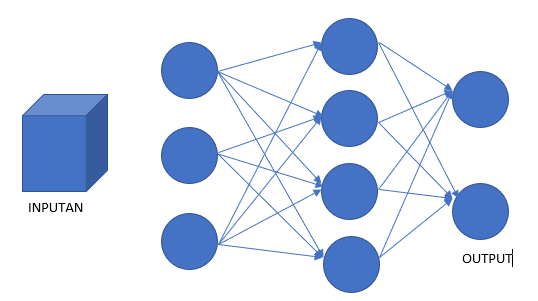
\includegraphics[width=0.7\textwidth]
      {figures/cokro/c114}}
      \caption{Ilustrasi Konsep dasar neural network}
      \label{c114}
      \end{figure}

\item Jelaskan konsep pembobotan  dalam neural network. dilengkapidengan ilustrasi gambar. \par
pembobotan dalam neural network yaitu digunakan untuk membedakan objek inputan atau variabel inputan untuk AI misalkan apel dan jeruk digunakan untuk variabel inputan maka dibuat pembobotan anatara kedua benda tersebut untuk menentukan output yang pasti dari inputan yang dilakukan untuk lebih jelasnya dapat dilihat pada gambar. \ref{c115}

\begin{figure}[!htbp]
      \centering{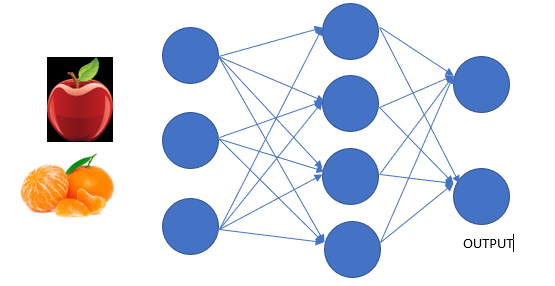
\includegraphics[width=0.7\textwidth]
      {figures/cokro/c115}}
      \caption{Ilustrasi Konsep pembobotan pada neural network}
      \label{c115}
      \end{figure}

\item Jelaskan konsep aktifitas dalam neural network. dilengkapi dengan ilustrasi gambar.\par

cara aktifitas dalam neural network dilakukan terhadap input pada neural network inputan tersebut dimasukan kepada fungsi pada mesin misalkan fungsi tanh(x) sehingga di hasilkanlah output yang sesuai dengan fungsi tersebut. untuk lebih jelasnya dapat dilihat pada gambar \ref{c116}

\begin{figure}[!htbp]
      \centering{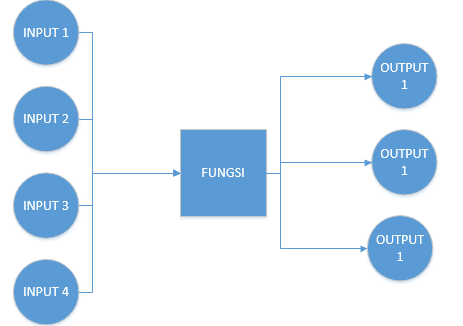
\includegraphics[width=0.7\textwidth]
      {figures/cokro/c116}}
      \caption{Gambar yang dibaca hasil plotnya}
      \label{c116}
	   \end{figure}

\item Jelaskan cara membaca hasil plot dari MFCC dilengkapi dengan ilustrasi gambar. \par
cara membaca hasil ploting dari MFCC yaitu tentukan terlebih dahulu batas minimal Hz dari gelombang suara dan batas maksimal dari suara tersebut. kemudian warna yang paling pekat merupakan hasil dari pengolahan data tersebut misalkan muncul warna orange pekat di bagian bawah dan orange muda di bagian atas yang berarti suara tersebut kuat bagian basnya dan biasanya juga antara warna yang pekat tersebut ada jarak. untuk lebih jelasnya dapat di lihat pada gambar \ref{c117} berikut.

\begin{figure}[!htbp]
      \centering{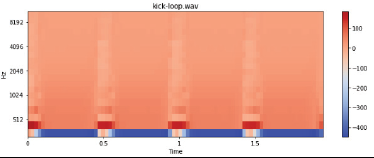
\includegraphics[width=0.7\textwidth]
      {figures/cokro/c117}}
      \caption{Ilustrasi Cara Membaca Hasil Plot}
      \label{c117}
      \end{figure}

\item Jelaskan apa itu one-hot encoding, dilengkapi dengan ilustrasi kode atau gambar.\par
one-hot encoding merupakan pemberian nilai pada suatu variabel jika nilai itu iya maka nilainya satu dan jika tidak maka nilainya nol untuk lebih jelasnya dapat dilihat pada gambar \ref{c118} tersebut

\begin{figure}[!htbp]
      \centering{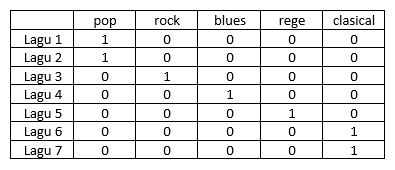
\includegraphics[width=0.7\textwidth]
      {figures/cokro/c118}}
      \caption{Ilustrasi Konsep one-hot encoding}
      \label{c118}
      \end{figure}

\item Jelaskan apa dari np.unique dan to\_categorical dalam kode program, dilengkapi dengan ilustrasi atau gambar.\par
digunakan untuk membuat array sedangkan  to\_categorical digunakan untuk membuat matrix baui itu 64 bit atau 32 bit. untuk contoh gambarnya dapat dilihat pada gambar \ref{c119} dan gambar \ref{c120}

\begin{figure}[!htbp]
      \centering{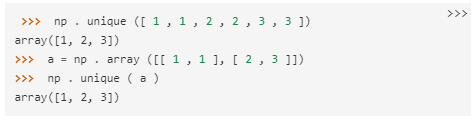
\includegraphics[width=0.7\textwidth]
      {figures/cokro/c119}}
      \caption{Ilustrasi  np.unique}
      \label{c119}
      \end{figure}

\begin{figure}[!htbp]
      \centering{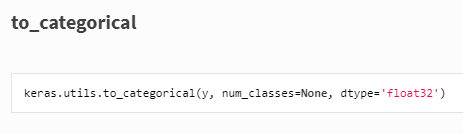
\includegraphics[width=0.7\textwidth]
      {figures/cokro/c120}}
      \caption{Ilustrasi to\_categorical}
      \label{c120}
      \end{figure}

\item Jelaskan apa fungsi dari Sequential dalam kode program, dilengkapi dengan ilustrasi atau gambar. \par
sequential adalah prosesperbandingan setiap elemen satu persatu mulai dari dari objek pertama hingga yang di tuju atau jika mencari angka 100 maka sequential akan membagi bagian misalnya dari satu sampai 20 dan seterusnya sampai mendapat nilai seratus. untuk lebih jelasnya dapat dilihat gambar \ref{c}  berikut:

\begin{figure}[!htbp]
      \centering{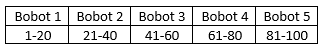
\includegraphics[width=0.5\textwidth]
      {figures/cokro/c121}}
      \caption{Ilustrasi Konsep pembobotan pada neural network}
      \label{c121}
      \end{figure}

\end{enumerate}

\section{Fathi Rabbani / 1164074}
\subsection{Teori}
\begin{enumerate}
\item Kenapa file suara harus dilakukan MFCC
\subitem MFCC digunakan untuk mengidentifikasi jenis suara yang dimasukan seperti suara lagu, hujan atau pun suara yang tidak dapat didengar oleh telinga manusia yaitu Ultrasonik, sehingga dibutuhkan penggunaan MFCC untuk memproses data tersebut agar dapat dibaca oleh manusia. ilustrasi untuk MFCC dapat dilihat pada gambar \ref{fig1}

\begin{figure}[!htbp]
      \centering{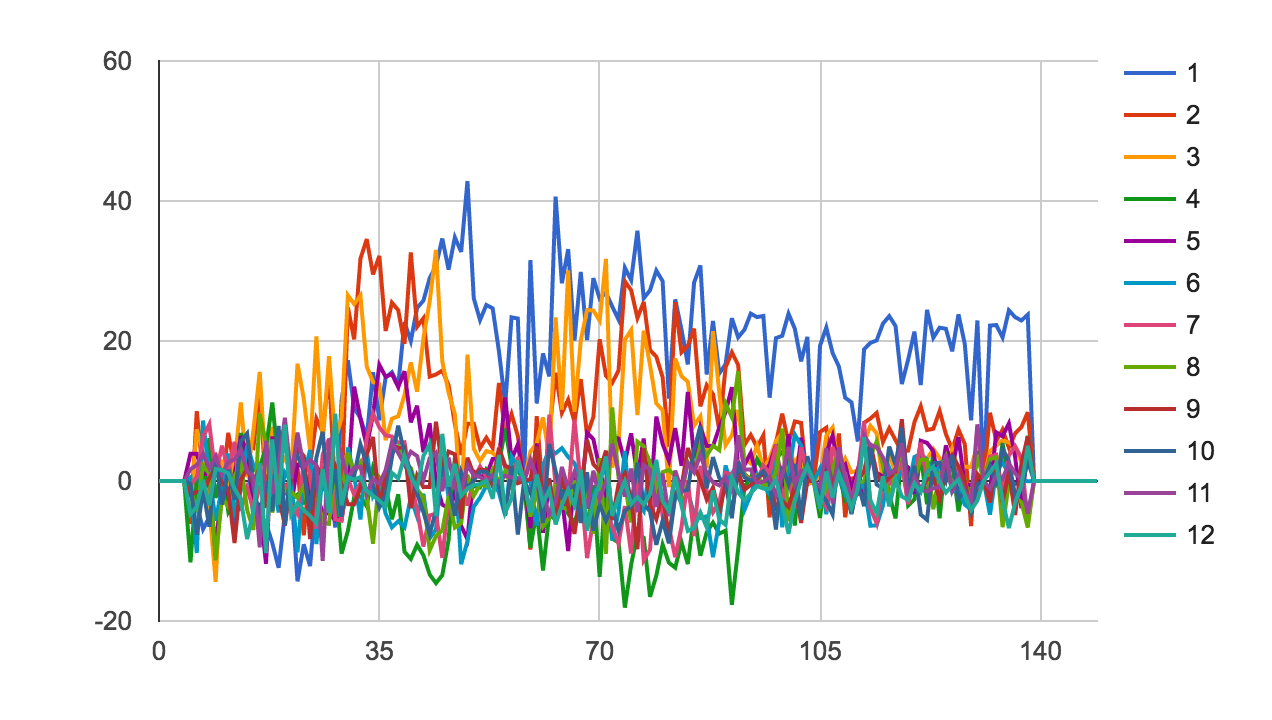
\includegraphics[width=0.5\textwidth]{figures/fathi/chapter6/hari1/1}}
      \caption{Ilustrasi MFCC}
      \label{fig1}
\end{figure}

\item Konsep dasar Neural Network
\subitem Neural Network sebenarnya mengadopsi dari kemampuan otak manusia yang mampu memberikan stimulasi/rangsangan, melakukan proses, dan memberikan output. Output diperoleh dari variasi stimulasi dan proses yang terjadi di dalam otak manusia.
ilustrasi Neural Network dapat dilihat pada gambar \ref{fig2}

\begin{figure}[!htbp]
      \centering{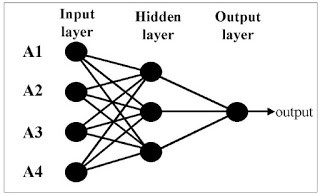
\includegraphics[width=0.5\textwidth]{figures/fathi/chapter6/hari1/2}}
      \caption{Ilustrasi Neural Network}
      \label{fig2}
\end{figure}

\item Konsep Pembobotan dalam Neural Network
\subitem konsep pembobotan dalam neural network digunakan untuk membedakan data satu dengan data lainnya, sebagai contoh dapat dilihat pada gambar \ref{fig3}. dimana data inputan yang masuk adalah 2 data yaitu "anjing" dan "kucing" yang diolah dengan proses membandingkan data dan diolah melalui pembobotan sehingga menampilkan hasil output.

\begin{figure}[!htbp]
      \centering{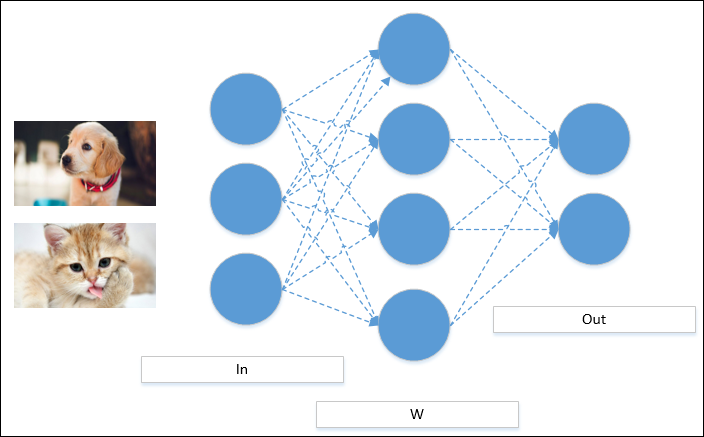
\includegraphics[width=0.5\textwidth]{figures/fathi/chapter6/hari1/3}}
      \caption{Ilustrasi pembobotan Neural Network}
      \label{fig3}
\end{figure}

\item Konsep Aktifasi dalam Neural Network
\subitem dalam Neural Network fungsi aktifasi meliputi inputan dan diproses sehingga menghasilkan Output nilai yang diharapkan, dengan menggunakan persepsi alur cara penyampaian informasi pada jaringan syaraf otak. ilustrasi dapat dilihat pada gambar \ref{fig4}

\begin{figure}[!htbp]
      \centering{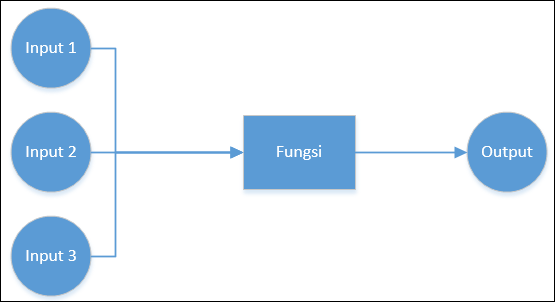
\includegraphics[width=0.5\textwidth]{figures/fathi/chapter6/hari1/4}}
      \caption{Ilustrasi fungsi aktifasi Neural Network}
      \label{fig4}
\end{figure}

\item cara membaca hasil PLOT dari MFCC

\begin{figure}[!htbp]
      \centering{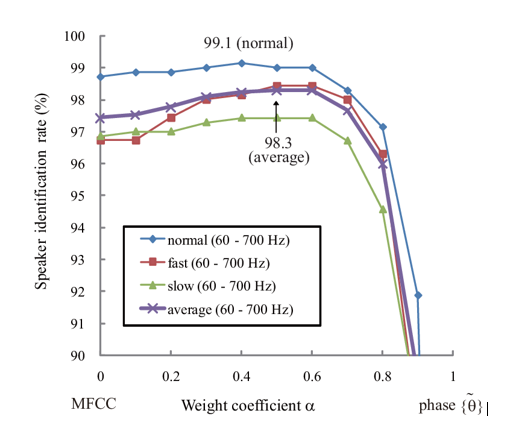
\includegraphics[width=0.5\textwidth]{figures/fathi/chapter6/hari1/5}}
      \caption{Ilustrasi Membaca nilai Plot dari MFCC}
      \label{fig5}
\end{figure}

\item One-hot Encoding
\subitem penggunaan One-hot Encoding adalah dengan membaca data yang memiliki nilai 1 sebagai nilai tinggi atau bisa disebut juga sebagai nilai positif dan 0 sebagai nilai rendah yang bermakna juga sebagai nilai negatif. ilustrasi dapat dilihat pada gambar \ref{fig6}

\begin{figure}[!htbp]
      \centering{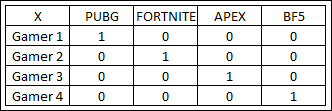
\includegraphics[width=0.5\textwidth]{figures/fathi/chapter6/hari1/6}}
      \caption{Ilustrasi One-hot Encoding}
      \label{fig6}
\end{figure}

\item fungsi dari np.unique dan to\_categorial dalam Code Program
\subitem fungsi dari NP.UNIQUE dalah untuk membuat data elemen menjadi nilai yang bersifat unik dalam artian (Array), ilustrasi dapat dilihat pada gambar \ref{fig7}

\begin{figure}[!htbp]
      \centering{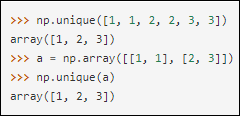
\includegraphics[width=0.5\textwidth]{figures/fathi/chapter6/hari1/7}}
      \caption{Ilustrasi np.unique}
      \label{fig7}
\end{figure}

\subitem sedangkan perintah to\_categorial adalah untuk membuat data integer yang terdeteksi untuk diubah menjadi data matrix biner. ilustrasi dapat dilihat pada gambar \ref{fig8}

\begin{figure}[!htbp]
      \centering{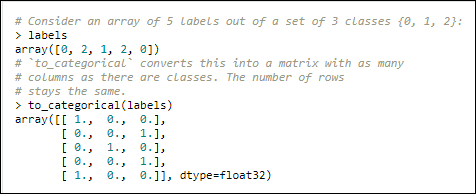
\includegraphics[width=0.5\textwidth]{figures/fathi/chapter6/hari1/8}}
      \caption{Ilustrasi to\_categorial}
      \label{fig8}
\end{figure}

\item fungsi dari Sequential
\subitem fungsi dari Sequential dari code program adalah untuk membagi data - data agar dapat dianalisis oleh sistem lebih mudah, misalkan dari data 100 dibagi prosesnya menjadi 4 yaitu 25 perproses, seperti yang terdapat pada gambar \ref{fig9} sehingga hasil yang didapatkan akan lebih baik lagi.

\begin{figure}[!htbp]
      \centering{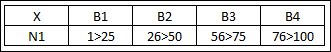
\includegraphics[width=0.5\textwidth]{figures/fathi/chapter6/hari1/9}}
      \caption{Ilustrasi fungsi Sequential}
      \label{fig9}
\end{figure}
\end{enumerate}